\section{Procedimiento de compilación}
La compilación de \texttt{OpuntiaOS} se llevó a cabo en la distribución 
\texttt{Ubuntu 22.04.3 LTS}.



Para comenzar con la construcción del sistema es necesario haber realizado las
instalaciones mencionadas en la \autoref{sec:reqPrevios}, según la arquitectura.
	

\subsection{ARM}
	El procedimiento debe seguirse como lo menciona el archivo \texttt{docs/build.md} del repositorio, en la sección \textit{Building OS}, en este caso:
	\begin{center}
		\ttfamily
		./gn\_gen.sh --target\_arch arm.
	\end{center}
	
	A continuación se muestra el flujo de instrucciones utilizado para la construcción:
	\begin{figure}[ht]
		\centering
		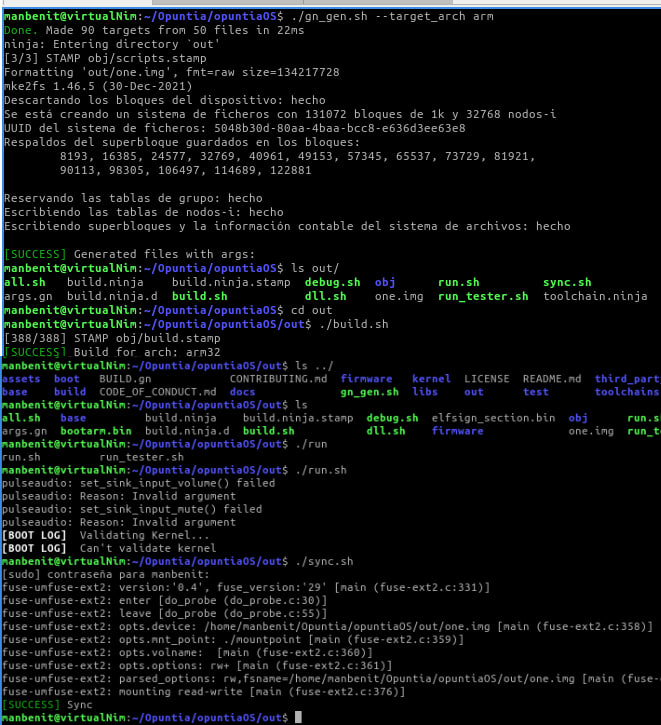
\includegraphics[scale=0.6]{buildArm.jpg}
		\caption{
			Construcción de la imagen de \texttt{OpuntiaOS} para \texttt{ARM}
			\label{fig:buildArm}
		}
	\end{figure}
	\begin{figure}[ht]
		\centering
		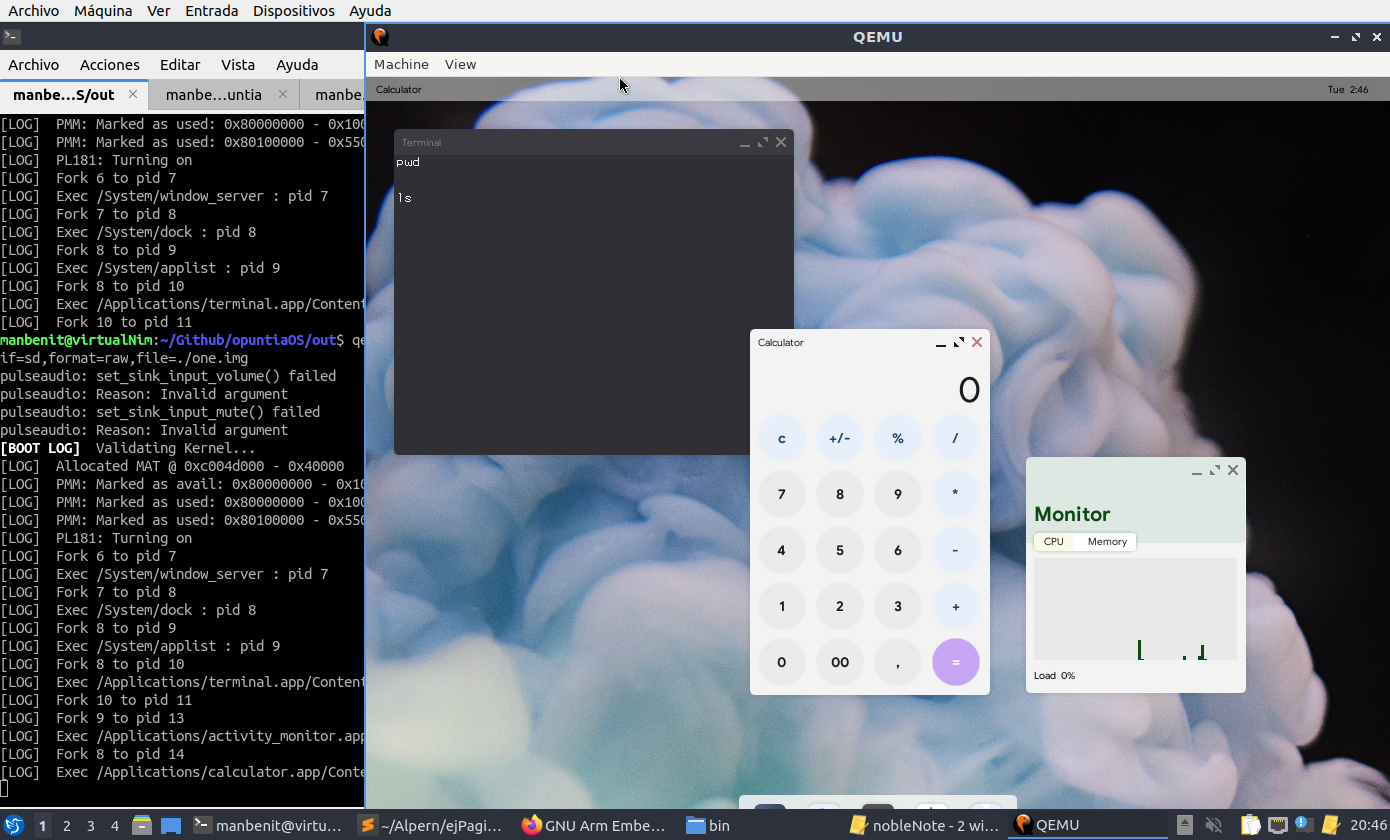
\includegraphics[scale=0.25]{primerARM.png}
		\caption{
			Arranque de la imagen de \texttt{OpuntiaOS} para \texttt{ARM}
			\label{fig:buildArm_res}
		}
	\end{figure}

	\textbf{NOTA}: Es importante ejecutar la sincronización (\texttt{sync.sh}) antes de 
	ejecutar el sistema (\texttt{run.sh}), si no se hace de esta forma, no terminan de sincronizarse los archivos con la imagen y el sistema se mostrará como muestra la \autoref{fig:armNoInit}.
	\begin{figure}[ht]
		\centering
		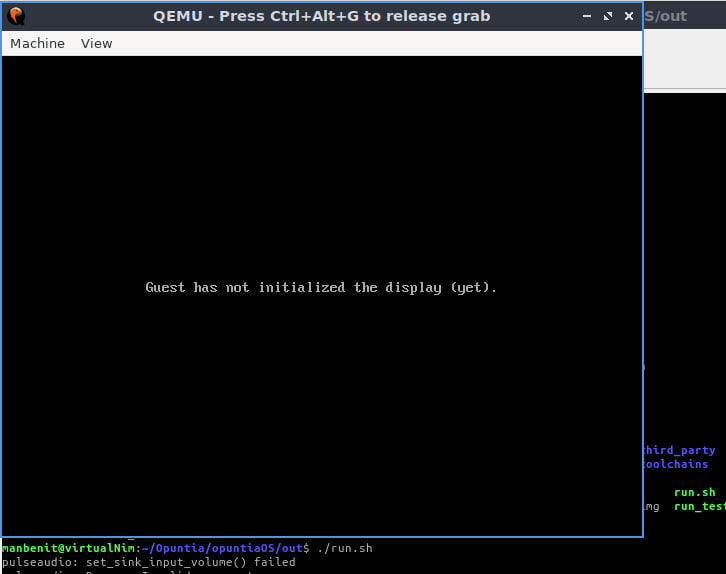
\includegraphics[scale=0.49]{armNoInit.jpg}
		\caption{
			Arranque de la imagen de \texttt{OpuntiaOS} para \texttt{ARM} si no se sincronizan los archivos.
			\label{fig:armNoInit}
		}
	\end{figure}





\newpage
\subsection{x86}
	El procedimiento debe seguirse como lo menciona el archivo \texttt{docs/build.md} del repositorio, en la sección \textit{Building OS}, en este caso:
	\begin{center}
		\ttfamily
		./gn\_gen.sh --target\_arch x86.
	\end{center}
	
	A continuación se muestra el flujo de instrucciones utilizado para la construcción:
	\begin{figure}[ht]
		\centering
		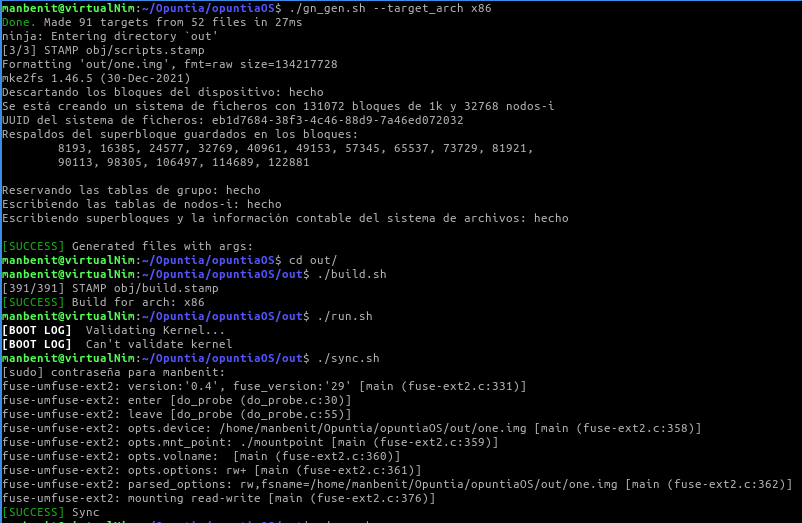
\includegraphics[scale=0.4]{buildx86.png}
		\caption{
			Construcción de la imagen de \texttt{OpuntiaOS} para \texttt{x86}
			\label{fig:buildx86}
		}
	\end{figure}
	\begin{figure}[ht]
		\centering
		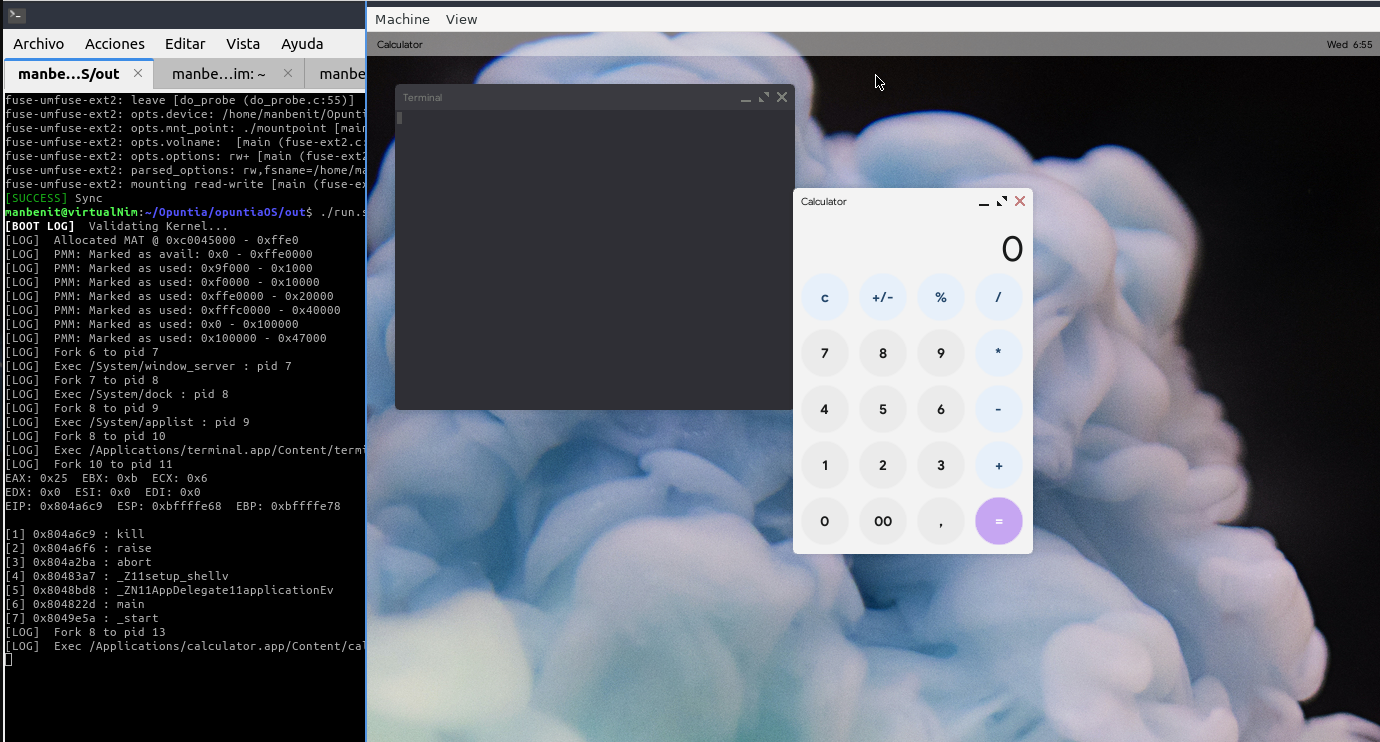
\includegraphics[scale=0.25]{primerx86.png}
		\caption{
			Arranque de la imagen de \texttt{OpuntiaOS} para \texttt{x86}
			\label{fig:buildx86_res}
		}
	\end{figure}
	
	\textbf{NOTA}: Es importante ejecutar la sincronización (\texttt{sync.sh}) antes de 
	ejecutar el sistema (\texttt{run.sh}), si no se hace de esta forma, no terminan de sincronizarse los archivos con la imagen y el sistema se mostrará como muestra la \autoref{fig:x86NoInit}.
	\begin{figure}[ht]
		\centering
		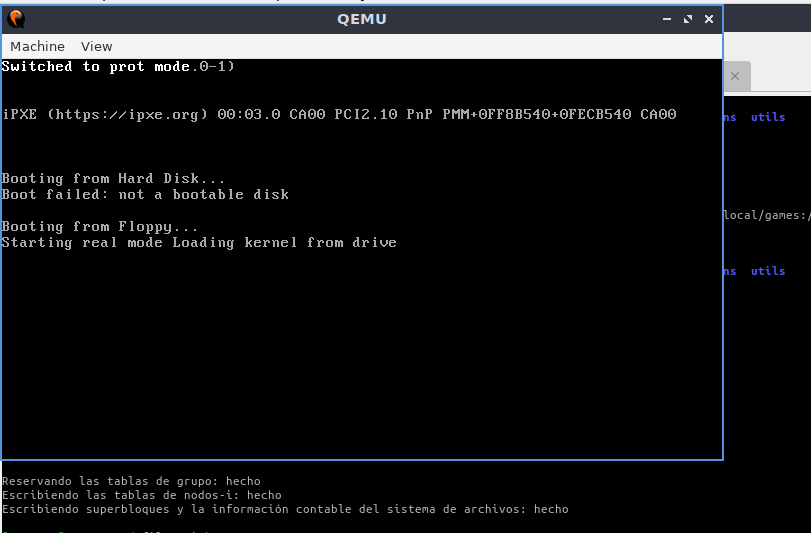
\includegraphics[scale=0.45]{x86NoInit.png}
		\caption{
			Arranque de la imagen de \texttt{OpuntiaOS} para \texttt{x86} si no se sincronizan los archivos.
			\label{fig:x86NoInit}
		}
	\end{figure}


















